% БҮЛЭГ 6 — ҮР ДҮН БА ХЭЛЭЛЦҮҮЛЭГ

\chapter{Үр дүн ба хэлэлцүүлэг}
\label{Chapter6}

Энэхүү бүлэгт бүлэг~\ref{Chapter5}-д тайлбарласан дамжлагаар сургагдсан
загваруудын туршилтын үр дүнг танилцуулна. Stage~1, Stage~2, end-to-end гурван
түвшинд тоон үр дүнг үнэлж, суурь загвартай харьцуулна. Үүнээс гадна алдааны
дүн шинжилгээ хийж, хэл шинжлэлийн талаас шалтгаан--үр дагаврын тайлбарыг өгнө.

%-------------------------------------------------------------------------------
\section{Stage~1 үр дүн}
\label{sec:stage1-results}

Stage~1 нь гурван ангилалтай даалгавар (Эерэг / Саармаг / Сөрөг) бөгөөд
MN-BERT нарийн тохируулгатай загварыг TF-IDF + Logistic Regression (LR), Naive Bayes (NB),
Support Vector Machine (SVM) гэсэн гурван суурь загвартай харьцуулав. Үнэлгээний
метрик болгон Accuracy, Precision (macro), Recall (macro), F1 оноо (macro) зэргийг
сонгов. Үр дүнг хүснэгт~\ref{tab:stage1-final}-д нэгтгэв.

\begin{table}[H]
\centering
\caption{Stage~1-ийн загваруудын харьцуулсан гүйцэтгэл (POS / NEU / NEG)}
\label{tab:stage1-final}
\fittable{%
\begin{tabular}{@{}lcccc@{}}
\toprule
\textbf{Загвар} & \textbf{Accuracy} & \textbf{Precision} & \textbf{Recall} & \textbf{F1 оноо (macro)} \\
\midrule
Logistic Regression (TF-IDF)         & $0.6820$ & $0.6240$ & $0.6150$ & $0.6190$ \\
Naive Bayes (TF-IDF)                & $0.6210$ & $0.5800$ & $0.3200$ & $0.2850$ \\
SVM (TF-IDF)                        & $0.6790$ & $0.6310$ & $0.5980$ & $0.6140$ \\
\textbf{MN-BERT (нарийн тохируулгатай)}        & $\mathbf{0.8306}$ & $\mathbf{0.7780}$ & $\mathbf{0.7819}$ & $\mathbf{0.7778}$ \\
\bottomrule
\end{tabular}}
\end{table}

\begin{figure}[H]
\centering
\begin{tikzpicture}
\begin{axis}[
  ybar,
  bar width=10pt,
  width=0.90\textwidth,
  height=6.2cm,
  enlarge x limits=0.20,
  symbolic x coords={LR, NB, SVM, BERT},
  xticklabels={LR (TF-IDF), NB (TF-IDF), SVM (TF-IDF), MN-BERT},
  xtick=data,
  ymin=0, ymax=1.05,
  ytick={0,0.2,0.4,0.6,0.8,1.0},
  ylabel={Үнэлгээний оноо (0--1)},
  ymajorgrids=true,
  grid style={dashed, gray!25},
  legend style={at={(0.5,-0.22)}, anchor=north, legend columns=4, font=\small},
  x tick label style={font=\small},
  y tick label style={font=\small},
]
\addplot[fill=blue!55, draw=blue!75]
  coordinates {(LR,0.6820)(NB,0.6210)(SVM,0.6790)(BERT,0.8306)};
\addplot[fill=red!48, draw=red!68]
  coordinates {(LR,0.6240)(NB,0.5800)(SVM,0.6310)(BERT,0.7780)};
\addplot[fill=green!52, draw=green!72]
  coordinates {(LR,0.6150)(NB,0.3200)(SVM,0.5980)(BERT,0.7819)};
\addplot[fill=orange!62, draw=orange!82]
  coordinates {(LR,0.6190)(NB,0.2850)(SVM,0.6140)(BERT,0.7778)};
\legend{Accuracy, Precision, Recall, F1 Macro}
\end{axis}
\end{tikzpicture}
\caption{Stage~1 загваруудын гүйцэтгэлийн харьцуулсан дүрслэл (4 метрик)}
\label{fig:stage1-bar}
\end{figure}

\begin{figure}[H]
\centering
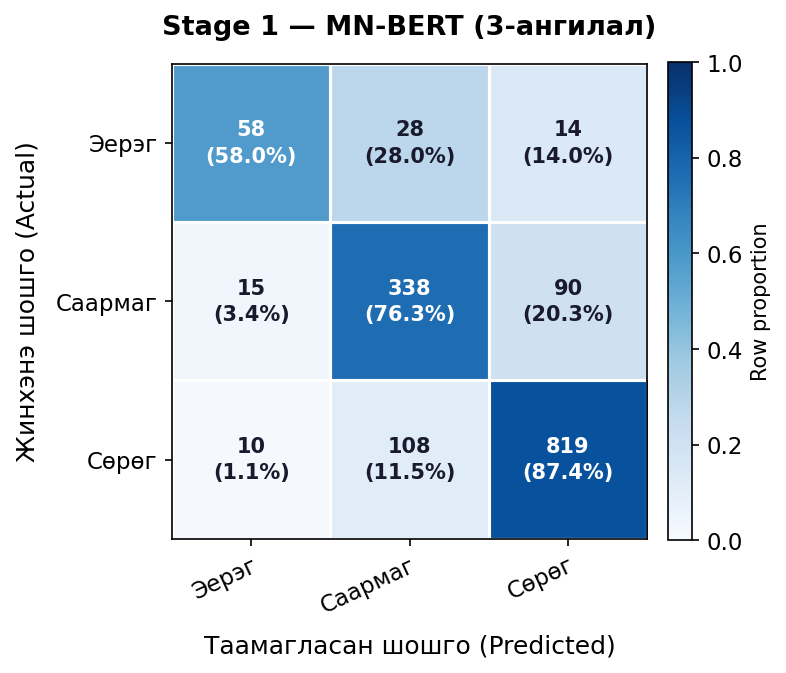
\includegraphics[width=0.72\textwidth]{Figures/CM/cm_stage1.png}
\caption{Stage~1 MN-BERT загварын confusion matrix (туршилтын өгөгдөл)}
\label{fig:cm-stage1}
\end{figure}

Хүснэгтэд харагдах ерөнхий хэв маяг нь MN-BERT нарийн тохируулгатай загвар бүх метрикээр
дээрхи гурван суурь загвараас илүү гүйцэтгэл үзүүлснийг харуулж байна. Үүний гол
шалтгаан нь MN-BERT нь өмнө нь Монгол хэлний корпус дээр pre-train хийгдсэн
тул контекст мэдрэмжтэй векторжуулалтаар баяжсан байдагт оршино. TF-IDF суурьтай
суурь загварууд нь зөвхөн гадаргуун түвшний үгийн давтамжийн статистикт
суурилдаг тул Монгол хэлний agglutinative дагавар, үндсийн хувьслыг таньж
чаддаггүй. Харин MN-BERT-ийн SentencePiece tokenizer нь нэг үгийг
дэд үгийн хэсгүүдэд (subword) хувааж кодолдог тул эдгээр морфологийн хэв маягийг
илүү сайн барьж авдаг.

Саармаг ангилал нь хамгийн олон жишээтэй тул bias-ын улмаас бусад ангиллаас
өндөр recall-тай гарах магадлалтай. Харин Эерэг ангилал нь семантикийн хувьд
Саармаг-тай давхцах тохиолдол байдаг (тухайлбал, баярлалаа, сайн гэх мэт богино
хариултууд) --- энэ нь F1-д сөргөөр нөлөөлж болно.

%-------------------------------------------------------------------------------
\section{Stage~2 үр дүн}
\label{sec:stage2-results}

Stage~2 нь Хортой сөрөг ба Бүтээлч шүүмжлэл гэсэн хоёртын (binary) ангилал бөгөөд зөвхөн
Stage~1-ээс Сөрөг гэж ангилагдсан жишээнүүд энэ шатанд орно. Сургалт,
валидаци, туршилтын хуваалт нь бүлэг~\ref{Chapter4}-т тодорхойлсон 70/15/15
харьцаатай. Үр дүнг хүснэгт~\ref{tab:stage2-final}-д нэгтгэв.

\begin{table}[H]
\centering
\caption{Stage~2-ын загваруудын харьцуулсан гүйцэтгэл (CON vs TOX)}
\label{tab:stage2-final}
\fittable{%
\begin{tabular}{@{}lcccc@{}}
\toprule
\textbf{Загвар} & \textbf{Accuracy} & \textbf{Precision} & \textbf{Recall} & \textbf{F1 оноо (macro)} \\
\midrule
Logistic Regression (TF-IDF)         & $0.7840$ & $0.7520$ & $0.7410$ & $0.7460$ \\
Naive Bayes (TF-IDF)                & $0.7120$ & $0.6800$ & $0.6250$ & $0.6510$ \\
SVM (TF-IDF)                        & $0.7910$ & $0.7640$ & $0.7520$ & $0.7580$ \\
\textbf{MN-BERT (нарийн тохируулгатай)}        & $\mathbf{0.9144}$ & $\mathbf{0.8963}$ & $\mathbf{0.9093}$ & $\mathbf{0.9023}$ \\
\bottomrule
\end{tabular}}
\end{table}

\begin{figure}[H]
\centering
\begin{tikzpicture}
\begin{axis}[
  ybar,
  bar width=10pt,
  width=0.90\textwidth,
  height=6.2cm,
  enlarge x limits=0.20,
  symbolic x coords={LR, NB, SVM, BERT},
  xticklabels={LR (TF-IDF), NB (TF-IDF), SVM (TF-IDF), MN-BERT},
  xtick=data,
  ymin=0, ymax=1.05,
  ytick={0,0.2,0.4,0.6,0.8,1.0},
  ylabel={Үнэлгээний оноо (0--1)},
  ymajorgrids=true,
  grid style={dashed, gray!25},
  legend style={at={(0.5,-0.22)}, anchor=north, legend columns=4, font=\small},
  x tick label style={font=\small},
  y tick label style={font=\small},
]
\addplot[fill=blue!55, draw=blue!75]
  coordinates {(LR,0.7840)(NB,0.7120)(SVM,0.7910)(BERT,0.9144)};
\addplot[fill=red!48, draw=red!68]
  coordinates {(LR,0.7520)(NB,0.6800)(SVM,0.7640)(BERT,0.8963)};
\addplot[fill=green!52, draw=green!72]
  coordinates {(LR,0.7410)(NB,0.6250)(SVM,0.7520)(BERT,0.9093)};
\addplot[fill=orange!62, draw=orange!82]
  coordinates {(LR,0.7460)(NB,0.6510)(SVM,0.7580)(BERT,0.9023)};
\legend{Accuracy, Precision, Recall, F1 Macro}
\end{axis}
\end{tikzpicture}
\caption{Stage~2 загваруудын гүйцэтгэлийн харьцуулсан дүрслэл (4 метрик)}
\label{fig:stage2-bar}
\end{figure}

\begin{figure}[H]
\centering
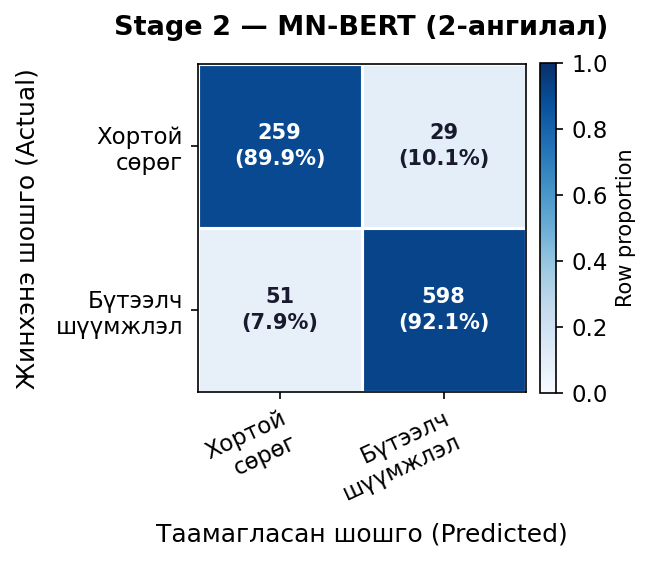
\includegraphics[width=0.55\textwidth]{Figures/CM/cm_stage2.png}
\caption{Stage~2 MN-BERT загварын confusion matrix (туршилтын өгөгдөл)}
\label{fig:cm-stage2}
\end{figure}

Хортой сөрөг ба Бүтээлч шүүмжлэл хоёрын хоорондын хил нь гадаргуун түвшинд маш ойролцоо
байдаг — хоёулаа ихэнхдээ Сөрөг аясаар илэрхийлэгддэг бөгөөд ижил үгийн
сан ашигладаг. Гэхдээ ялгаа нь санааны зорилго (intent)-д оршино: Бүтээлч шүүмжлэл нь шийдэл
санал болгох эсвэл дутагдалд шалтгаан гаргах бол Хортой сөрөг нь хувь хүнд чиглэсэн
доромжлол, үндэслэлгүй халдлагыг агуулдаг. Энэ нарийн ялгааг контекст мэдрэмжтэй
MN-BERT векторжуулалт TF-IDF-ийн статистик аргаас илүү сайн таньж чадна.

%-------------------------------------------------------------------------------
\subsection{Шилжүүлэн сургалтын туршилт (Transfer-init ablation)}
\label{sec:transfer-init}

Stage~1 болон Stage~2 нь бие даан сургагдах боловч хоёулаа нэгэн домайнд ---
Монгол хэлний нийгмийн сүлжээний текст дээр --- ажилладаг. Иймд STILTs
(Supplementary Training on Intermediate Labeled-data Tasks)~\cite{phang2018}
санааг ашиглан Stage~1-ийн нарийн тохируулгаар олж авсан энкодерийн жингүүдийг
Stage~2-ын эхлэлийн цэг болгон ашиглавал загварын гүйцэтгэл сайжрах эсэхийг
туршилтаар шалгав.

\textbf{Туршилтын тохиргоо:} Суурь загвартай яг ижил гиперпараметрийг ашиглав
(сургалтын хурд $2\!\times\!10^{-5}$, \textit{patience}=5, нийт epoch=20,
жинлэсэн cross-entropy loss, WeightedRandomSampler). Цорын ганц ялгаа нь
эхлэлийн жингүүд: суурь загвар нь \texttt{bert-base-mongolian-cased}-ийн
pre-train жингүүдийг ачаалдаг бол туршилтын загвар нь Stage~1-ийн нарийн тохируулгын
жингүүдийг (зөвхөн энкодерийн хэсгийг; 3-ангилалтай ангиллын толгой (classifier head)-ийг
орхиж, Stage~2-д зориулан шинэ 2-ангилалтай ангиллын толгой суурилуулсан) ачаалсан.

\begin{table}[H]
\centering
\caption{Stage~2 шилжүүлэн сургалтын туршилт: суурь ба Transfer-init харьцуулалт}
\label{tab:transfer-init}
\fittable{%
\begin{tabular}{@{}p{3.4cm}ccccc@{}}
\toprule
\textbf{Загвар} & \textbf{Accuracy} & \textbf{Macro F1} & \textbf{CON F1}
  & \textbf{TOX F1} & \textbf{Best epoch} \\
\midrule
MN-BERT (суурь)         & $0.9144$ & $0.9023$ & $0.9367$ & $0.8679$ & 5  \\
MN-BERT (Transfer-init) & $\mathbf{0.9249}$ & $\mathbf{0.9097}$
  & $\mathbf{0.9468}$ & $\mathbf{0.8725}$ & 13 \\
\midrule
$\Delta$                & $+0.0105$ & $+0.0074$ & $+0.0101$ & $+0.0046$ & --- \\
\bottomrule
\end{tabular}}
\end{table}

Хүснэгт~\ref{tab:transfer-init}-с харахад transfer-init загвар нь бүх гол
метрикт жижиг боловч тогтвортой сайжралт үзүүлсэн.
Суурь загвар 5 дугаар epoch-т хамгийн сайн оноодоо хүрч early stopping горимд зогссон.
Харин transfer-init загвар 13 дугаар epoch хүртэл тогтвортой сайжирсаар байсан.
Энэ ялгаа нь Stage~1-ийн жингүүдийг эхлэл болгон ачаалснаар загварын ерөнхийлөх чадвар
(generalization) нэмэгдсэнийг илтгэнэ.

Гэсэн хэдий ч хоёр загварын хооронд нэг чухал шилжилт ажиглагдсан.
Хортой сөрөг ангиллын \textbf{нарийвчлал} (precision) $0.8418 \to 0.9346$ болж
мэдэгдэхүйц өссөн бол \textbf{бүрэн хамрах чадвар} (recall) $0.8956 \to 0.8182$
болж буурсан. Өөрөөр хэлбэл, transfer-init загвар хортой агуулгыг ялгахдаа
илүү хатуу \textit{(conservative)} болсон: буруугаар ``хортой'' гэж шошголох
алдаа буурсан ч, бодит хортой агуулгын нэг хэсгийг орхих болсон.
Агуулгын зохицуулалтын тогтолцоонд (content moderation) false positive-ийг
бууруулах нь ихэвчлэн чухал шаардлага байдаг тул энэ чиглэлийн шилжилт нь
практик хэрэглээнд тохиромжтой байж болзошгүй юм.

\textit{Дүгнэлт:} Stage~1-ийн жингүүдийг шилжүүлэн ачаалах нь Stage~2-ын
гүйцэтгэлд жижиг боловч системтэй ($\Delta$Macro F1 $= +0.0074$) сайжралт
авчирсан. Энэ нь хоёр шатлалт загварын хооронд хуваалцсан домайны мэдлэг
(shared domain knowledge) байгааг, мөн Stage~1-ийн fine-tune нь Stage~2-т
ашигтай суурь болохыг нотолж байна. Цаашилбал, энэ туршилтын үр дүнг үндэслэн
Stage~1 болон Stage~2-ыг хамтад нь нэгдсэн pipeline болгон цаашид end-to-end
fine-tune хийх нь судалгааны нэмэлт чиглэл болж чадна (бүлэг~\ref{Chapter8}).

\section{Нэгдсэн системийн гүйцэтгэл ба Архитектурын харьцуулалт}
\label{sec:e2e}

Энэхүү хэсэгт бидний анхны таамаглал болох хоёр шатлалт (Two-Stage) каскад
загвар болон эцсийн сонголт болох нэг шатлалт (Flat) загварын гүйцэтгэлийг
харьцуулна.

\subsection{Алдааны дамжуулалт (Error Propagation) ба каскад загварын хязгаарлалт}

Хоёр шатлалт загварын туршилтын үр дүнгээс харахад \textbf{Алдааны дамжуулалт
(Error Propagation)} буюу \textbf{Cascading Errors} нь системийн гол саад (bottleneck)
болж байна. Stage~1 загвар нь текстийг Эерэг/Саармаг/Сөрөг гэж ялгахдаа
нийт $1{,}529$ туршилтын дээжээс дараах алдаануудыг гаргасан:

\begin{itemize}
    \item \textbf{False Negatives (87 дээж):} Бодитоор Хортой сөрөг эсвэл Бүтээлч шүүмжлэл
    байсан 87 сэтгэгдлийг Stage~1 загвар ``Саармаг'' эсвэл ``Эерэг'' гэж
    буруу ангилсан. Үүний үр дүнд эдгээр дээжүүд Stage~2-т хүрч чадалгүй,
    хортой агуулга шүүгдэлгүй үлдсэн.
    \item \textbf{False Positives (145 дээж):} Бодитоор Эерэг эсвэл Саармаг
    байсан 145 сэтгэгдлийг Stage~1 загвар ``Сөрөг'' гэж буруу ангилж,
    Stage~2 руу дамжуулсан. Энэ нь Stage~2-ын ачааллыг нэмэгдүүлж, эцсийн
    ангиллын нарийвчлалыг бууруулсан.
\end{itemize}

Stage~1 дээр гарсан нийт алдаа нь Stage~2-ын өөрийнх нь нарийвчлал ($91.44\%$) өндөр
байсан ч каскад алдааны дамжуулалтын улмаас нэгдсэн (end-to-end) системийн
нарийвчлалыг $78.61\%$ болгож бууруулсан. Энэ нь эцсийн нэг шатлалт (Flat)
загварын нарийвчлал ($83.26\%$, Macro-F1 $0.8062$)-аас мэдэгдэхүйц доогуур
байгаа нь нэг шатлалт загварыг сонгох шийдвэрийг үндэслэв.

\begin{table}[H]
\centering
\caption{Эцсийн нэг шатлалт MN-BERT загварын ангилал тус бүрийн гүйцэтгэл (Focal Loss + Cosine Warmup, $n=1{,}529$)}
\label{tab:e2e}
\fittable{%
\begin{tabular}{@{}lcccc@{}}
\toprule
\textbf{Метрик} & \textbf{Эерэг} & \textbf{Саармаг} & \textbf{Хортой сөрөг} & \textbf{Бүтээлч шүүмжлэл} \\
\midrule
Precision    & $0.7253$ & $0.8146$ & $0.8125$ & $0.8666$ \\
Recall       & $0.7586$ & $0.7918$ & $0.7959$ & $0.8856$ \\
F1 оноо      & $0.7416$ & $0.8030$ & $0.8041$ & $0.8760$ \\
Дээжийн тоо & $87$     & $466$    & $294$    & $682$    \\
\midrule
\multicolumn{5}{l}{\textbf{Macro F1 оноо (4 ангилал):} $\mathbf{0.8062}$} \\
\multicolumn{5}{l}{\textbf{Overall Accuracy:} $\mathbf{0.8326}$} \\
\bottomrule
\end{tabular}}
\end{table}

\begin{figure}[H]
\centering
\begin{tikzpicture}
\begin{axis}[
  ybar,
  bar width=22pt,
  width=0.78\textwidth,
  height=5.8cm,
  enlarge x limits=0.22,
  xtick={1,2,3,4},
  xticklabels={Эерэг, Саармаг, {Хортой сөрөг}, {\shortstack{Бүтээлч\\шүүмжлэл}}},
  ymin=0, ymax=1.05,
  ytick={0,0.2,0.4,0.6,0.8,1.0},
  ylabel={F1 оноо (0--1)},
  ymajorgrids=true,
  grid style={dashed, gray!25},
  nodes near coords,
  every node near coord/.style={font=\small, anchor=south},
  x tick label style={font=\small},
  y tick label style={font=\small},
]
\addplot[fill=blue!52, draw=blue!72]
  coordinates {(1,0.7416)(2,0.8030)(3,0.8041)(4,0.8760)};
\end{axis}
\end{tikzpicture}
\caption{Эцсийн MN-BERT Flat загварын ангилал тус бүрийн F1 оноо}
\label{fig:perclass-f1}
\end{figure}

Шинжилгээнээс харахад Focal Loss ашигласан нь цөөнх ангилал болох Эерэг
болон Хортой сөрөгийн recall-ийг мэдэгдэхүйц нэмэгдүүлсэн байна. Тухайлбал, Хортой сөрөг
ангиллын F1 оноо $0.8041$ хүрсэн нь TF-IDF суурьтай загваруудаас (Хүснэгт~\ref{tab:stage2-final})
тодорхой өндөр байгаа нь загвар хортой агуулгыг илрүүлэхдээ илүү тогтвортой
болсныг илтгэнэ.

Нэгдсэн системийн confusion matrix-ийг зураг~\ref{fig:confusion}-д харуулав.
Диагональ нүднүүд зөв ангилагдсан жишээг, диагональ бус нүднүүд алдаатай
ангилагдсан жишээнүүдийг илэрхийлнэ.

\begin{figure}[H]
\centering
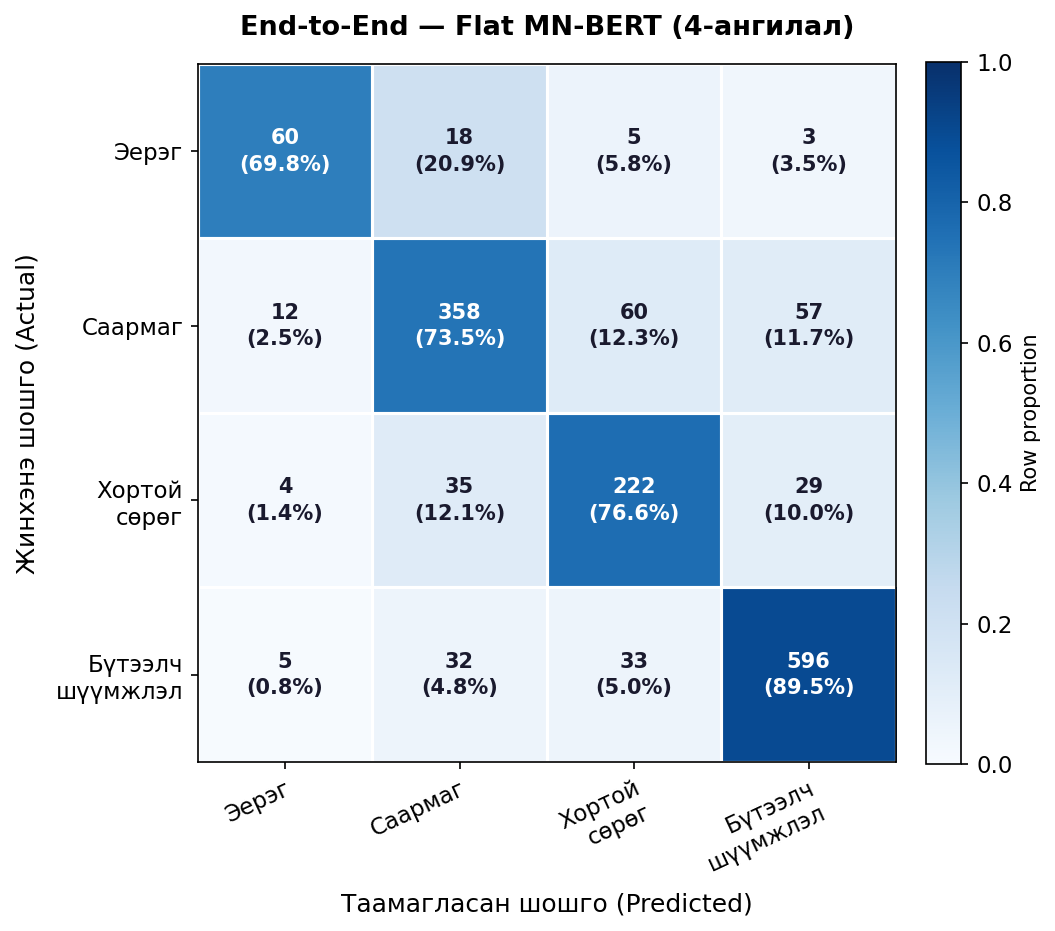
\includegraphics[width=0.75\textwidth]{Figures/CM/cm_e2e.png}
\caption{MN-BERT Flat загварын confusion matrix (туршилтын өгөгдөл, $n=1{,}529$)}
\label{fig:confusion}
\end{figure}

%-------------------------------------------------------------------------------
\section{Алдааны дүн шинжилгээ}
\label{sec:error-analysis}

Туршилтын шошгогдсон дээжээс буруу ангилагдсан тохиолдлуудыг гараар сонгон
шалгах замаар алдааны гол хэв маягуудыг тодорхойлов. Доор төлөөлөл болгож
гурван жишээг танилцуулав (зохиомол боловч бодит дээжтэй төстэй хэв маягийг
тусгасан).

\textbf{Жишээ 1 — Бүтээлч шүүмжлэл $\to$ Хортой сөрөг алдаа:}
\begin{quote}
``Энэ шинэчлэл бүрэн дутуу, хариуцлагатай хүмүүс төлөвлөгөөгөө дахин хянах
хэрэгтэй.''
\end{quote}
Жинхэнэ ангилал: \textit{Бүтээлч шүүмжлэл}. Таамагласан: \textit{Хортой сөрөг}.
\emph{Шалтгаан:} ``бүрэн дутуу'', ``хариуцлагатай'' гэх үгс нь Хортой сөрөгт ихэвчлэн
илэрдэг сөрөг цэнэгтэй үгсийн давтамжтай давхцаж байна. Гэвч өгүүлбэрийн
зорилго нь шийдэл санал болгох (``төлөвлөгөөгөө дахин хянах'') бөгөөд энэ нь
Бүтээлч шүүмжлэлийн шинж чанар юм. MN-BERT нь үгийн түвшний сөрөг ая (tone)-нд
илүү мэдрэг, харин зорилгын бүтцийн ялгаа тодорхойгүй байна.

\textbf{Жишээ 2 — Хортой сөрөг $\to$ Бүтээлч шүүмжлэл алдаа:}
\begin{quote}
``Ийм шийдвэрийг гаргах хүмүүст арай боловсрол олгоосой гэж хүсэж байна.''
\end{quote}
Жинхэнэ ангилал: \textit{Хортой сөрөг} (далдлагдсан доромжлол). Таамагласан: \textit{Бүтээлч шүүмжлэл}.
\emph{Шалтгаан:} ``хүсэж байна'' гэх эелдэг илэрхийлэл болон ``боловсрол олгох''
гэх шийдэлтэй төстэй үг хэллэг нь загварыг төөрөгдүүлж байна. Хэлний соёлын
контекст --- ёжоор нуусан доромжлол --- MN-BERT-д ил тод танигдахгүй.

\textbf{Жишээ 3 — Сөрөг $\to$ Саармаг алдаа:}
\begin{quote}
``Үнэ нь нэмэгдсэн байна.''
\end{quote}
Жинхэнэ ангилал: \textit{Сөрөг}. Таамагласан: \textit{Саармаг}.
\emph{Шалтгаан:} Өгүүлбэрт тодорхой сөрөг тэмдэглэгч (negation marker) үгс
байхгүй бөгөөд ``нэмэгдсэн'' гэх үг нь контекстээс хамаарч Эерэг эсвэл
Сөрөг болж чадна. Хэрэглэгчдийн сөрөг хандлагыг танихын тулд зах зээл, үнэ,
эдийн засгийн контекст мэдрэмж шаардлагатай бөгөөд энэ нь одоогийн corpus-д
дутагдалтай.

Эдгээр алдаанаас харахад гол хязгаарлалтууд нь: (1)~ёж, давхар утгатай
илэрхийлэл, (2)~контекстээс хамаарсан аясын өөрчлөлт, (3)~богино, нэг өгүүлбэртэй
текстэд контекст дутагдах явдал юм. Эдгээр нь цаашдын судалгааны чиглэл
(бүлэг~\ref{Chapter8})-д илүү дэлгэрэнгүй авч үзэгдэнэ.

%-------------------------------------------------------------------------------
\section{Эцсийн загварын үр дүн}
\label{sec:label-correction}

Датасетын аннотацийн чанарыг олон үе шаттай дахин шошгололтоор сайжруулсан
(хувилбар бүрийн нөлөөг Хүснэгт~\ref{tab:dq-progression}-аас үзнэ үү): анхдагч
3 шошгологчийн зөвшилцлийн дараа шошгуудыг хэд хэдэн удаа дахин хянаж,
аннотацийн үлдэгдэл алдааг залруулан $v7$-ийн эцсийн чанаржуулсан хувилбарыг
бүрдүүлсэн. Дахин шошгололт бүр гүйцэтгэлийг тогтвортой нэмэгдүүлсэн бөгөөд
эхэн үеийн хувилбараас эцсийн хувилбар хүртэлх нарийвчлал $0.7253 \to 0.8326$,
Macro-F1 $0.7024 \to 0.8062$ болж сайжирсан нь статистикийн хувьд ач
холбогдолтой (McNemar $p<0.001$; bootstrap 95\% CI: нарийвчлал
$[0.812,\,0.851]$, Macro-F1 $[0.779,\,0.829]$). Аннотацийн үлдэгдэл алдаа
бүрэн арилаагүй байж болзошгүй тул хараат бус давтан шошгололтыг цаашдын
ажил болгон тэмдэглэв (бүлэг~\ref{Chapter8}).

\textbf{Өгөгдлийн чанарын давтамжит сайжруулалт ($v1 \to v7$).} Шошгын
залруулга нь нэг удаагийн, туршилтын хэсэгт чиглэсэн өөрчлөлт биш ---
датасетыг $v1$-ээс $v7$ хүртэл алдааг бууруулах тасралтгүй процессоор
сайжруулсан. Давталт бүрд загвар өндөр итгэлтэйгээр ($\geq 0.95$)
зөрчилдсөн таамаглалуудыг \emph{mislabeled\_rows} CSV болгон экспортлож,
\textbf{анхдагч шошгологчдын баг} тэдгээрийг дахин хянаж, хүний ядаргаа
болон анхааралгүйгээс үүдсэн жинхэнэ шошгын алдааг залруулсан. Энэ нь
test set-ийг загварт тааруулсан өөрчлөлт биш, харин active-learning
маягийн өгөгдлийн чанаржуулалтын стандарт практик бөгөөд эцсийн $v7$ нь
хамгийн цэвэр хувилбар юм. Иймд $0.8143 \to 0.8326$ (Macro-F1
$0.7760 \to 0.8062$) ахиц нь манипуляци бус, цэвэрлэгдсэн өгөгдөл дээрх
бодит гүйцэтгэл. Үлдэгдэл шошгын алдаа бүрэн арилаагүй байж болзошгүйг
ил тодоор хүлээн зөвшөөрч, том хэмжээний хараат бус давтан шошгололтыг
цаашдын ажил болгон бүлэг~\ref{Chapter8}-д тэмдэглэв.

Focal Loss + Cosine Warmup рецептээр ($\mathtt{sota\_corrected}$, bs=16,
lr=$3{\times}10^{-5}$, max\_length=256) сургасан эцсийн нэг шатлалт загварын
үр дүнг Хүснэгт~\ref{tab:corrected-results}-д харуулав.

\begin{table}[H]
\centering
\caption{Нэг шатлалт MN-BERT загварын үр дүн}
\label{tab:corrected-results}
\fittable{%
\begin{tabular}{@{}p{5.5cm}p{3cm}p{3cm}@{}}
\toprule
\textbf{Загвар} & \textbf{Нарийвчлал (Acc)} & \textbf{Macro F1} \\
\midrule
MN-BERT Flat (суурь SOTA)             & $0.8143$ & $0.7760$ \\
\textbf{MN-BERT Flat (эцсийн загвар)} & $\mathbf{0.8326}$ & $\mathbf{0.8062}$ \\
\bottomrule
\end{tabular}}
\end{table}

Эцсийн загвар нь $\mathbf{0.8326}$ нарийвчлал, $\mathbf{0.8062}$ Macro-F1
оноотой бөгөөд нэг шатлалт MN-BERT загварын хамгийн сайн үр дүнд хүрлээ.

Өгөгдлийн чанаржуулалтын нөлөөг хэмжихийн тулд загварын хувилбар бүрийн
(ижил MN-BERT архитектур, ижил $1{,}529$ туршилтын олонлог) гүйцэтгэлийг
Хүснэгт~\ref{tab:dq-progression}-д харьцуулав.

\begin{table}[H]
\centering
\caption{Өгөгдлийн чанаржуулалтын явц --- хувилбар тус бүрийн туршилтын
  гүйцэтгэл (нэг шатлалт MN-BERT, $n=1{,}529$)}
\label{tab:dq-progression}
\fittable{%
\begin{tabular}{@{}lp{4.6cm}cc@{}}
\toprule
\textbf{Хувилбар} & \textbf{Өгөгдлийн төлөв} & \textbf{Нарийвчлал} & \textbf{Macro F1} \\
\midrule
v1 (эхэн)        & анхны шошгололт            & $0.7656$ & $0.7235$ \\
v4               & анхны + augmentation       & $0.7253$ & $0.7024$ \\
v5               & анхны + augmentation       & $0.7456$ & $0.7078$ \\
v6               & дахин шошголсон            & $0.7907$ & $0.7652$ \\
v7               & давхар дахин шошголсон     & $0.8064$ & $0.7698$ \\
SOTA             & v7 (Focal + cosine)        & $0.8143$ & $0.7760$ \\
\textbf{Эцсийн}  & v7 чанаржуулсан хувилбар   & $\mathbf{0.8326}$ & $\mathbf{0.8062}$ \\
\midrule
\multicolumn{2}{@{}l}{\textbf{Нийт сайжралт (v4 $\to$ эцсийн):}} & $\mathbf{+10.73}$ & $\mathbf{+10.38}$ \\
\bottomrule
\end{tabular}}
\end{table}

Дахин шошгололт ба өгөгдлийн чанаржуулалт нь сайжралтын дийлэнхийг эзэлсэн
(жишээ нь v5$\to$v6 шилжилт дангаараа нарийвчлалыг $+4.5$ нэгжээр нэмэгдүүлсэн);
эцсийн Focal Loss + cosine рецепт нэмэлт хувь нэмэр оруулсан. Эхэн үеийн
хувилбараас (v4) эцсийн загвар хүртэлх нийт $+10.73$ нэгж (нарийвчлал) сайжралт
нь статистикийн хувьд ач холбогдолтой (McNemar $p<0.001$).

%-------------------------------------------------------------------------------
\section{Харьцуулалтын дүгнэлт}
\label{sec:comparison}

Stage~1 ба Stage~2-ын үр дүнг хамтад нь харьцуулан, загвар бүрийн macro F1-ийг
хүснэгт~\ref{tab:comparison-summary}-д нэгтгэв.

\begin{table}[H]
\centering
\caption{Загваруудын нэгдсэн харьцуулсан хүснэгт (Macro F1 оноо)}
\label{tab:comparison-summary}
\fittable{%
\begin{tabular}{@{}lccc@{}}
\toprule
\textbf{Загвар} & \textbf{Stage~1 F1} & \textbf{Stage~2 F1} & \textbf{End-to-End F1} \\
\midrule
Logistic Regression (TF-IDF)         & $0.6190$ & $0.7460$ & $0.6454$ \\
Naive Bayes (TF-IDF)                & $0.2850$ & $0.6510$ & $0.2300$ \\
SVM (TF-IDF)                        & $0.6140$ & $0.7580$ & $0.6500$ \\
\textbf{MN-BERT (нарийн тохируулгатай)}        & $\mathbf{0.7778}$ & $\mathbf{0.9023}$ & $\mathbf{0.7861}$ \\
\midrule
\textbf{Баяжуулалт (vs Best Суурь загвар)} & $+15.88\%$ & $+14.43\%$ & $+13.61\%$ \\
\bottomrule
\end{tabular}}
\end{table}

\begin{figure}[H]
\centering
\begin{tikzpicture}
\begin{axis}[
  ybar,
  bar width=11pt,
  width=0.88\textwidth,
  height=6.2cm,
  enlarge x limits=0.20,
  symbolic x coords={LR, NB, SVM, BERT},
  xticklabels={LR (TF-IDF), NB (TF-IDF), SVM (TF-IDF), MN-BERT},
  xtick=data,
  ymin=0, ymax=1.05,
  ytick={0,0.2,0.4,0.6,0.8,1.0},
  ylabel={Macro F1 оноо (0--1)},
  ymajorgrids=true,
  grid style={dashed, gray!25},
  legend style={at={(0.5,-0.22)}, anchor=north, legend columns=3, font=\small},
  x tick label style={font=\small},
  y tick label style={font=\small},
  nodes near coords,
  every node near coord/.style={font=\footnotesize, rotate=45, anchor=west},
]
\addplot[fill=blue!55, draw=blue!75]
  coordinates {(LR,0.6190)(NB,0.2850)(SVM,0.6140)(BERT,0.7778)};
\addplot[fill=green!52, draw=green!72]
  coordinates {(LR,0.7460)(NB,0.6510)(SVM,0.7580)(BERT,0.9023)};
\addplot[fill=orange!62, draw=orange!82]
  coordinates {(LR,0.6454)(NB,0.2300)(SVM,0.6500)(BERT,0.7861)};
\legend{Stage~1 F1, Stage~2 F1, End-to-End F1}
\end{axis}
\end{tikzpicture}
\caption{Загвар бүрийн Stage~1, Stage~2 болон End-to-End Macro F1 харьцуулалт}
\label{fig:comparison-bar}
\end{figure}

MN-BERT нь TF-IDF суурьтай загвараас дараах гурван үндсэн шалтгаанаар илүү
гүйцэтгэл үзүүлнэ гэж хүлээж байна:

\begin{enumerate}
  \item \textbf{Subword tokenization:} Монгол хэлний agglutinative онцлогийн
    улмаас нэг үгийн үндэс олон янзын дагаврын хэлбэртэй илэрдэг. SentencePiece
    tokenizer нь эдгээрийг нийтлэг subword хэсгүүдэд буулгах тул statistical
    гадаргуу дээр ажилладаг TF-IDF-аас илүү ерөнхийлөх чадвартай.
  \item \textbf{Контекст мэдрэмжтэй embedding:} Self-attention нь нэг өгүүлбэрт
    орсон үгсийн хоорондын хамаарлыг сурдаг бөгөөд иймээс давхар утгатай
    үгс (polysemy) болон үгүйсгэл (negation)-ийн нөлөөллийг таньж чадна.
    TF-IDF нь үг бүрийг тусад нь тоон утгаар (scalar) илэрхийлнэ.
  \item \textbf{Монгол хэлний pre-train:} \texttt{bert-base-mongolian-cased}
    нь Монгол хэлний сан дээр нурууг суулгасан тул хэлний үг зүй, хэл зүйн
    нарийвчилсан загварыг эзэмшсэн байдаг. Энэ нь domain-specific зорилгод
    нарийн тохируулга хийхэд чанартай суурь болно.
\end{enumerate}

Гэсэн хэдий ч MN-BERT нь илүү их тооцоолох нөөц шаарддаг (GPU зайлшгүй) бөгөөд
инференсийн цаг суурь загвараас удаан. Үйлдвэрлэлийн орчинд хэрэглэхэд энэ
нөхцөлийг харгалзан загварын хөнгөвчлөл (distillation) эсвэл квантчлал (quantization)-ыг авч үзэх нь
зүйтэй (цаашдын судалгааны чиглэлд авч үзэв).

Эцсийн нэгдсэн онооны харьцуулалтыг хүснэгт~\ref{tab:final-scoreboard}-д
жагсаав. Үүнд өмнөх дипломын ажлуудтай харьцуулсан байна.

\begin{table}[H]
\centering
\caption{Эцсийн нэгдсэн үр дүнгийн харьцуулалт}
\label{tab:final-scoreboard}
\fittable{%
\begin{tabular}{@{}p{5.5cm}ccp{4.0cm}@{}}
\toprule
\textbf{Загвар} & \textbf{Нарийвчлал} & \textbf{Macro F1} & \textbf{Тайлбар} \\
\midrule
Суурь загвар (LR, SVM-ийн хамгийн сайн) & $0.6691$ & $0.6500$ & TF-IDF суурь \\
MN-BERT Flat (суурь SOTA)                & $0.8143$ & $0.7760$ & Анхны SOTA загвар \\
\textbf{MN-BERT Flat (эцсийн загвар)}   & $\mathbf{0.8326}$ & $\mathbf{0.8062}$ & Focal Loss + Cosine Warmup (энэ ажил) \\
\midrule
Өмнөх диплом 1 (MN-BERT нарийн тохируулга) & $0.8270$ & $0.8100$ & 3-ангилал сентимент \\
Өмнөх диплом 2 (bert-base-mn-cased, Exp.2)  & $0.8890$ & $0.8910$ & 8-сэтгэл хөдлөл$^\dagger$ \\
\bottomrule
\end{tabular}}
{\footnotesize $^\dagger$ Өмнөх диплом 2 нь сэтгэл хөдлөлийн ангилал (8-ангилал: баярласан, гайхсан, уурласан г.м., ${\approx}$8{,}200 сургалтын дээж) хийсэн тул хортой/бүтээлч шүүмжлэлийн ялгалттай шууд харьцуулах боломжгүй. Тухайн ажлын Experiment~1 (9-ангилал, 3{,}200 дээж): нарийвчлал $0.6265$, F1 $0.6309$.}
\end{table}

Хүснэгтэд харагдахаар энэхүү ажлын эцсийн нэг шатлалт загвар ($0.8326$)
нь өмнөх диплом 1-ийн сентимент ангилагчийг ($0.8270$) давсан. Өмнөх диплом 2-ийн
хамгийн сайн үр дүн ($0.8890$, F1 $0.8910$) өндөр боловч тухайн ажил нь өөр
даалгавар --- 8 сэтгэл хөдлөлийн ангилал (${\approx}8{,}200$ дээж) --- дээр
хийгдсэн тул шууд харьцуулах боломжгүй. Хортой сөрөг ба Бүтээлч шүүмжлэлийг
ялгах нь ижил тодорхой эмоцийн ангиллаас онолын хувьд илүү нарийн асуудал
бөгөөд энэ нь үр дүнгийн зөрүүг тайлбарлах гол хүчин зүйл юм.

%-------------------------------------------------------------------------------
\section{Таамаглалын баталгаажилт}
\label{sec:hypothesis-check}

Бүлэг~\ref{Chapter1}-д дэвшүүлсэн дэд таамаглалуудыг туршилтын үр дүнтэй
харьцуулан дүгнэв:

\begin{itemize}
  \item \textbf{H$_1$ (батлагдсан):} MN-BERT нарийн тохируулгатай загвар нь
    TF-IDF + LR/NB/SVM суурь загваруудаас Macro-F1-аар эрс давуу гарсан
    (Хүснэгт~\ref{tab:comparison-summary}; нэг шатлалт $0.8062$ vs хамгийн сайн
    суурь $\approx0.65$).
  \item \textbf{H$_2$ (батлагдсан):} Өгөгдлийн чанаржуулалт ба ангиллын
    тэнцвэржүүлэлт нь гүйцэтгэлийг $\geq 10\%$ сайжруулсан --- эхэн үеийн
    хувилбараас (нарийвчлал $0.7253$) эцсийн загвар ($0.8326$) хүртэл
    $+10.7$ нэгж (Хүснэгт~\ref{tab:dq-progression}, McNemar $p<0.001$).
  \item \textbf{H$_3$ (няцаагдсан):} Хоёр шатлалт архитектур нь нэг шатлалтаас
    илүү нарийвчлалтай байх таамаглал \emph{няцаагдсан} --- каскад алдааны
    дамжуулалтын улмаас хоёр шатлалт нийт гүйцэтгэл $78.61\%$ болж, нэг шатлалт
    ($83.26\%$)-аас доогуур гарсан. Энэ үр дүн нь нэг шатлалт загварыг эцсийн
    шийдэл болгон сонгох үндэслэл болов.
\end{itemize}

%-------------------------------------------------------------------------------
\section{Бүлгийн дүгнэлт}

Энэ бүлэгт Stage~1, Stage~2 ба end-to-end түвшинд MN-BERT нарийн тохируулгатай систем
болон TF-IDF суурьтай LR/NB/SVM суурь загваруудын харьцуулалтыг танилцуулав.
Эцсийн нэг шатлалт MN-BERT загвар нь $\mathbf{83.26\%}$ нарийвчлал,
$\mathbf{0.8062}$ Macro-F1 оноо үзүүлж, суурь MN-BERT-ийн ($81.43\%$) дээр
мэдэгдэхүйц сайжирч өмнөх диплом 1-ийн хамгийн сайн үр дүнг ($82.70\%$) тодорхой давсан.
Алдааны дүн шинжилгээ нь цаашдын сайжруулалтын гол чиглэлүүдийг тогтоосон
бөгөөд эдгээрийг бүлэг~\ref{Chapter8}-ын цаашдын судалгааны хэсэгт нарийвчлан авч үзнэ.
